
\section{Question 3}
\label{part1}

\begin{itemize}
\item Using 20 links that have TimeMaps
\begin{itemize}
\item With $>= 20$ mementos
\item Have existed  $>= 2$ years (i.e., Memento-Datetime of “first memento” is April XX, 2013 or older)
\item Note: select from Q1/Q2 links, else choose them by hand
\end{itemize}
\item For each link, create a graph that shows Jaccard Distance, relative to the first memento, through time
\begin{itemize}
\item x-axis: continuous time, y-axis: Jaccard Distance relative to the first memento
\end{itemize}
\end{itemize}
\begin{figure}[ht]
	\begin{center}
		 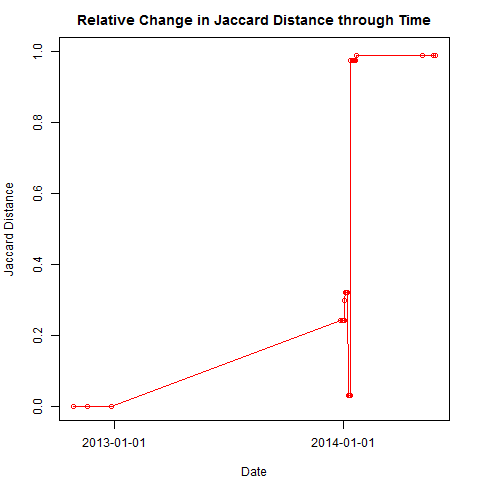
\includegraphics[scale=0.60]{url1}
		  \caption{Jaccard Distance relative to the first memento url1}
	 \end{center}
\end{figure}
\begin{figure}[ht]
	\begin{center}
		 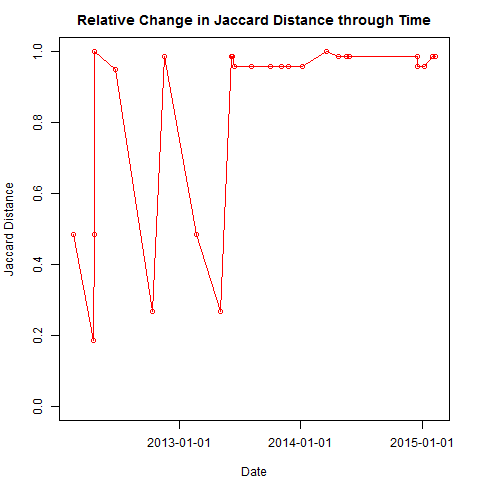
\includegraphics[scale=0.60]{url2}
		  \caption{Jaccard Distance relative to the first memento url2}
	 \end{center}
\end{figure}
\begin{figure}[ht]
	\begin{center}
		 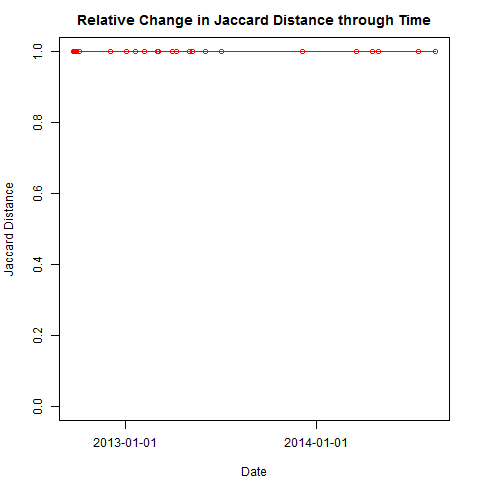
\includegraphics[scale=0.60]{url3}
		  \caption{Jaccard Distance relative to the first memento url3}
	 \end{center}
\end{figure}
\begin{figure}[ht]
	\begin{center}
		 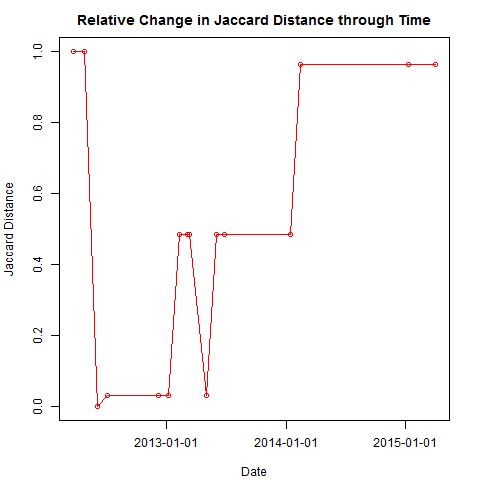
\includegraphics[scale=0.60]{url4}
		  \caption{Jaccard Distance relative to the first memento url4}
	 \end{center}
\end{figure}
\begin{figure}[ht]
	\begin{center}
		 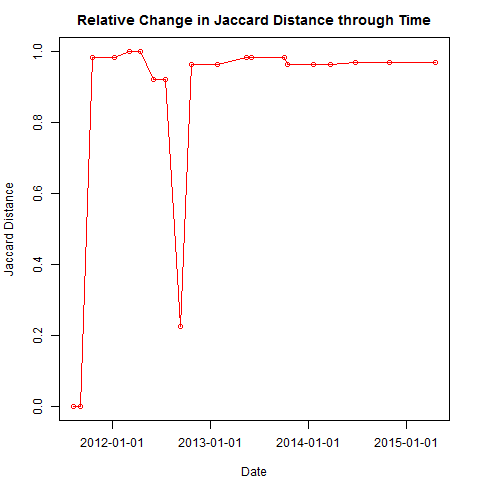
\includegraphics[scale=0.60]{url5}
		  \caption{Jaccard Distance relative to the first memento url5}
	 \end{center}
\end{figure}
\begin{figure}[ht]
	\begin{center}
		 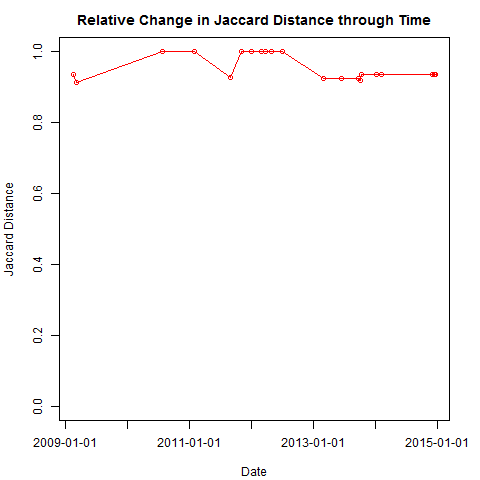
\includegraphics[scale=0.60]{url6}
		  \caption{Jaccard Distance relative to the first memento ur65}
	 \end{center}
\end{figure}
\begin{figure}[ht]
	\begin{center}
		 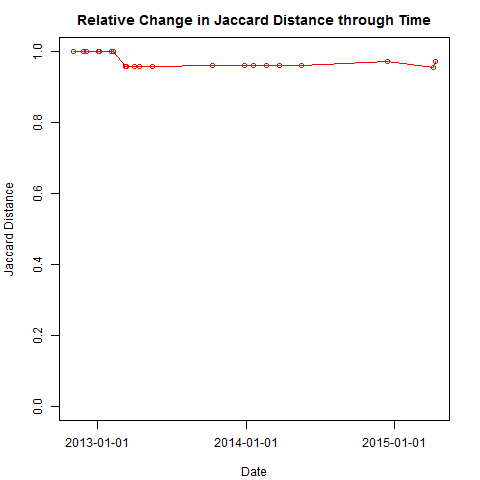
\includegraphics[scale=0.60]{url7}
		  \caption{Jaccard Distance relative to the first memento url7}
	 \end{center}
\end{figure}
\begin{figure}[ht]
	\begin{center}
		 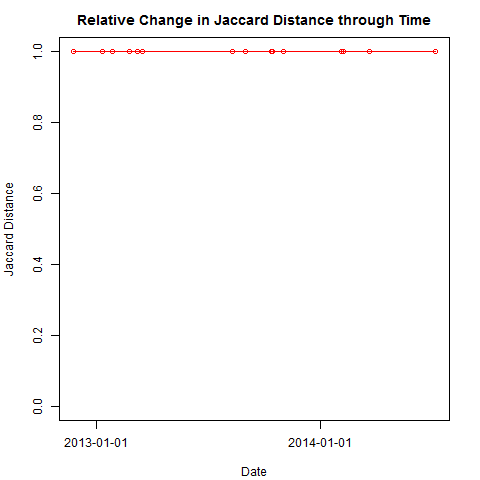
\includegraphics[scale=0.60]{url8}
		  \caption{Jaccard Distance relative to the first memento url8}
	 \end{center}
\end{figure}
\clearpage
\begin{figure}[ht]
	\begin{center}
		 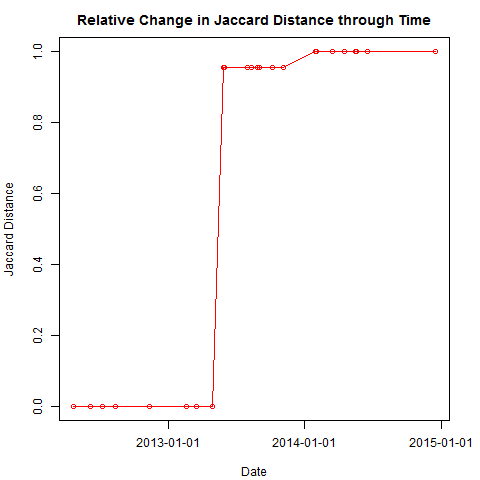
\includegraphics[scale=0.60]{url9}
		  \caption{Jaccard Distance relative to the first memento url9}
	 \end{center}
\end{figure}
\begin{figure}[ht]
	\begin{center}
		 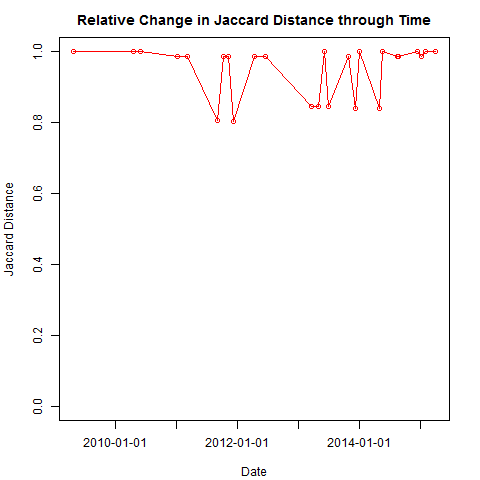
\includegraphics[scale=0.60]{url10}
		  \caption{Jaccard Distance relative to the first memento url10}
	 \end{center}
\end{figure}
\begin{figure}[ht]
	\begin{center}
		 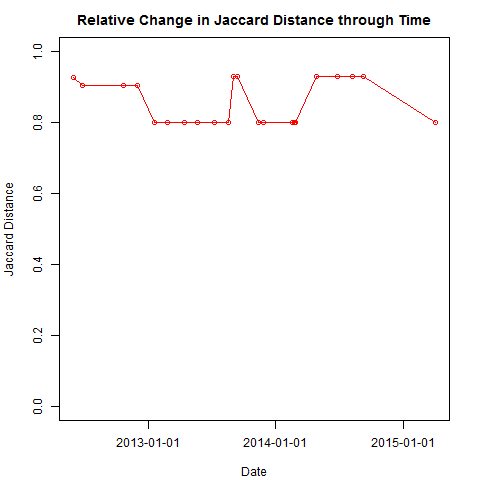
\includegraphics[scale=0.60]{url11}
		  \caption{Jaccard Distance relative to the first memento url11}
	 \end{center}
\end{figure}
\begin{figure}[ht]
	\begin{center}
		 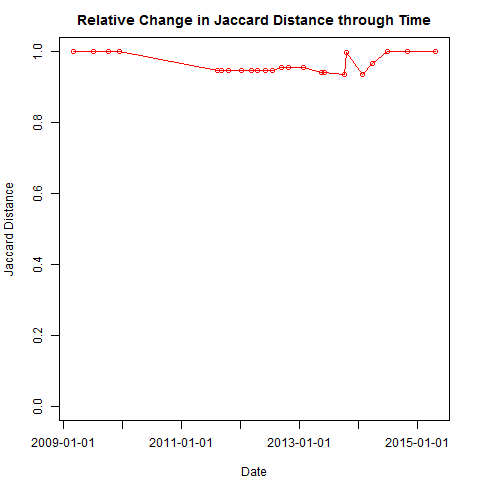
\includegraphics[scale=0.60]{url12}
		  \caption{Jaccard Distance relative to the first memento url12}
	 \end{center}
\end{figure}
\begin{figure}[ht]
	\begin{center}
		 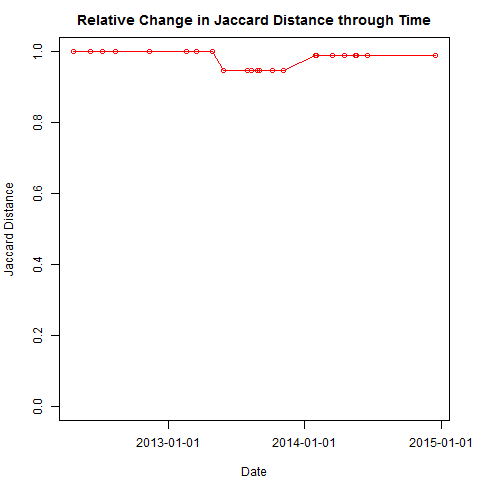
\includegraphics[scale=0.60]{url13}
		  \caption{Jaccard Distance relative to the first memento url13}
	 \end{center}
\end{figure}
\begin{figure}[ht]
	\begin{center}
		 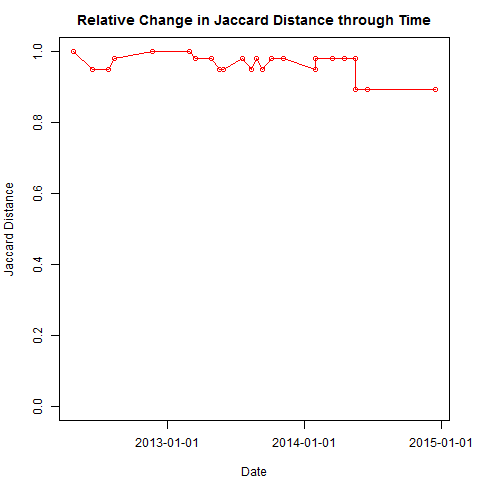
\includegraphics[scale=0.60]{url14}
		  \caption{Jaccard Distance relative to the first memento url14}
	 \end{center}
\end{figure}
\begin{figure}[ht]
	\begin{center}
		 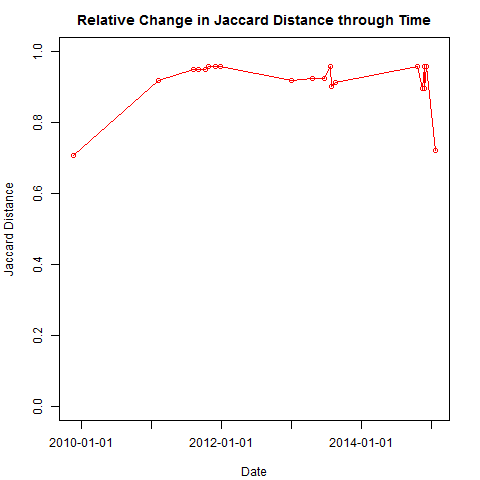
\includegraphics[scale=0.60]{url15}
		  \caption{Jaccard Distance relative to the first memento url15}
	 \end{center}
\end{figure}
\begin{figure}[ht]
	\begin{center}
		 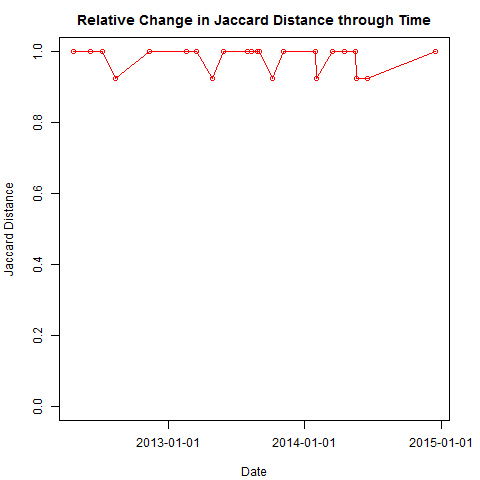
\includegraphics[scale=0.60]{url16}
		  \caption{Jaccard Distance relative to the first memento url16}
	 \end{center}
\end{figure}
\clearpage
\begin{figure}[ht]
	\begin{center}
		 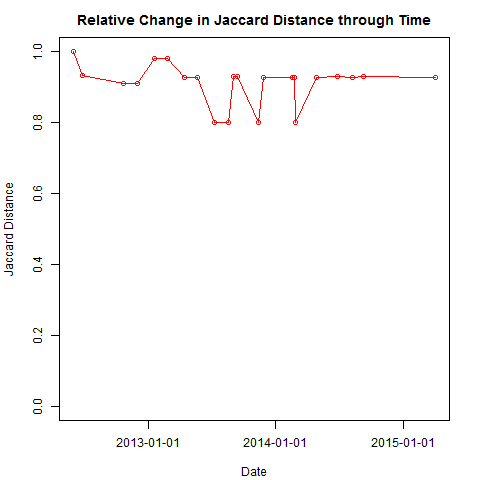
\includegraphics[scale=0.60]{url17}
		  \caption{Jaccard Distance relative to the first memento url17}
	 \end{center}
\end{figure}
\begin{figure}[ht]
	\begin{center}
		 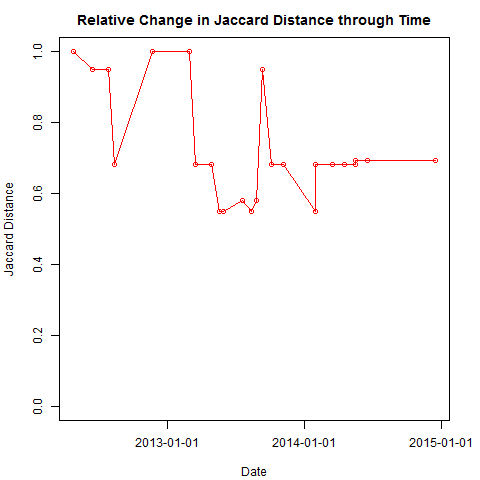
\includegraphics[scale=0.60]{url18}
		  \caption{Jaccard Distance relative to the first memento url18}
	 \end{center}
\end{figure}
\begin{figure}[ht]
	\begin{center}
		 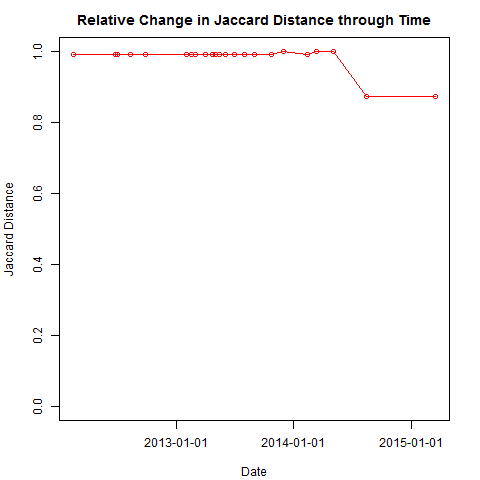
\includegraphics[scale=0.60]{url19}
		  \caption{Jaccard Distance relative to the first memento url19}
	 \end{center}
\end{figure}
\begin{figure}[ht]
	\begin{center}
		 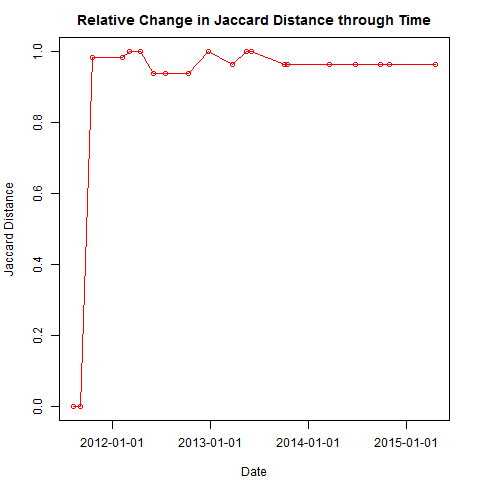
\includegraphics[scale=0.60]{url20}
		  \caption{Jaccard Distance relative to the first memento url20}
	 \end{center}
\end{figure}